%%%%%%%%%%%%%%%%%%%%%%%%%%%%%%%%%%%%%%%%%%%%%%%%%%%%%%%%%%%%%%%%%%%%%%%%
% Uni Duesseldorf
% Lehrstuhl fuer Datenbanken und Informationssysteme
% Vorlage fuer Bachelor-/Masterarbeiten
% Optimiert fuer den Original-Latex-Kompiler LATEX.EXE (LaTeX=>PS=>PDF)
%%%%%%%%%%%%%%%%%%%%%%%%%%%%%%%%%%%%%%%%%%%%%%%%%%%%%%%%%%%%%%%%%%%%%%%%
% Ueberarbeitung für pdflatex (LaTeX=>PDF)
%%%%%%%%%%%%%%%%%%%%%%%%%%%%%%%%%%%%%%%%%%%%%%%%%%%%%%%%%%%%%%%%%%%%%%%%
% Vorlage Changelog:
% 10.09.2015 (Matthias Liebeck): Nummerierung des Inhaltsverzeichnis nun römisch, Beispiel für einen Anhang eingebaut, \raggedbottom hinter sections eingefügt
% 11.07.2018 (Matthias Liebeck): Ersetzung des Bibliographiestils, Einsatz von Biber
% 04.09.2018 (Matthias Liebeck):
%   * Bibtex: unnötige Bibtexfelder beim Rendern ausblenden (thx @ Markus Brenneis)
%   * ngerman: "et al." im BibTeX für drei oder mehr Autoren
%   * Neuer Befehl \sectionforcestartright: Sections immer rechts beginnen (thx @ Philipp Grawe)
%   * ngerman: Deutsche Anführungszeichen im Literaturverzeichnis (thx @ Markus Brenneis)
%   * ngerman: Deutsche Anführungszeichen im Literaturverzeichnis (thx @ Markus Brenneis)
%%%%%%%%%%%%%%%%%%%%%%%%%%%%%%%%%%%%%%%%%%%%%%%%%%%%%%%%%%%%%%%%%%%%%%%%
%%%% BEGINN EINSTELLUNG FUER DIE ARBEIT. UNBEDINGT ERFORDERLICH! %%%%%%%
%%%%%%%%%%%%%%%%%%%%%%%%%%%%%%%%%%%%%%%%%%%%%%%%%%%%%%%%%%%%%%%%%%%%%%%%
% Geben Sie Ihren Namen hier an:
\newcommand{\bearbeiter}{Julian Robert Ullrich}

% Geben Sie hier den Titel Ihrer Arbeit an:
\newcommand{\titel}{Actor-Critic Reinforcement Learning With Experience Replay}

% Geben Sie das Datum des Beginns und Ende der Bachelorarbeit ein:
\newcommand{\beginndatum}{25. Juli 2018}
\newcommand{\abgabedatum}{25.~Oktober~2018}

% Geben Sie die Namen des Erst- und Zweitgutachters an:
\newcommand{\erstgutachter}{Univ.-Prof. Dr. S. Harmeling}
\newcommand{\zweitgutachter}{Univ.-Prof. Dr. M. Leuschel}
\newcommand{\betreuer}{Julius Ramakers}

% Falls Sie die Arbeit zweiseitig ausdrucken wollen,
% benutzen Sie die folgende Zeile mit
% \AN fuer zweiseitigen Druck
% \AUS fuer einseitigen Druck
\newcommand{\zweiseitig}{\AN}

% Falls Sections immer rechts beginnen sollen. Gerade für Masterarbeiten
% interessant. Bei kurzen Bachelorarbeiten eher weniger zu verwenden.
\newcommand{\sectionforcestartright}{\AUS}
%\newcommand{\sectionforcestartright}{\AN}

% Falls die Arbeit in englischer Sprache verfasst 
% werden soll, dann benutzen Sie die folgende Zeile mit
% englisch fuer englische Sprache
% deutsch fuer deutsche Sprache
\newcommand{\sprache}{englisch}

% Hier wird eingestellt, ob es sich bei der Arbeit um eine Bachelor- 
% oder Masterarbeit handelt (unpassendes auskommentieren!):
\newcommand{\arbeit}{Bachelorarbeit}
%~ \newcommand{\arbeit}{Masterarbeit}


%%%%%%%%%%%%%%%%%%%%%%%%%%%%%%%%%%%%%%%%%%%%%%%%%%%%%%%%%%%%%%%%%%%%%%%%
%%%% ENDE EINSTELLUNGEN %%%%%%%%%%%%%%%%%%%%%%%%%%%%%%%%%%%%%%%%%%%%%%%%
%%%%%%%%%%%%%%%%%%%%%%%%%%%%%%%%%%%%%%%%%%%%%%%%%%%%%%%%%%%%%%%%%%%%%%%%

% Die folgende Zeile NICHT EDITIEREN oder loeschen


%%%%%%%%%%%%%%%%%%%%%%%%%%%%%%%%%%%%%%%%%%%%%%%%%%%%%%%%%%%
% Obere Titelmakros. Editieren Sie diese Datei nur, wenn
% Sie sich ABSOLUT sicher sind, was Sie da tun!!!
% (Z.B. zum Abaendern der BA-Vorlage in eine MA-Vorlage)
% Uni Duesseldorf
% Lehrstuhl fuer Datenbanken und Informationssysteme
% Version 2.2 - 2.3.2010
%%%%%%%%%%%%%%%%%%%%%%%%%%%%%%%%%%%%%%%%%%%%%%%%%%%%%%%%%%%
\newcommand{\AN}{twoside}
\newcommand{\AUS}{}
%\newcommand{\englisch}{}
%\newcommand{\deutsch}{\usepackage[german]{babel}}

%% Die folgenden auskommentierten Optionen dienen der automatischen
%% Erkennung des Latex-Kompilers und dem Setzen der davon abhängigen
%% Einstellungen. Bei Problem z.B. mit dem Einbinden von verschiedenen
%% Grafiktypen bei Verwendung von PdfLatex oder Latex, einfach die
%% verschiedenen \usepackage(s) ausprobieren. (Mit diesen Einstellungen
%% funktionierte diese Vorlage bei der Verwenundg von latex.exe als
%% Kompiler bei den meisten Studierenden.)

%\newif\ifpdf \ifx\pdfoutput\undefined
%\pdffalse % we are not running pdflatex
%\else
%\pdfoutput=1 % we are running pdflatex
%\pdfcompresslevel=9 % compression level for text and image;
%\pdftrue \fi

\documentclass[11pt,a4paper, \zweiseitig]{article}



%\usepackage[iso]{umlaute}
\usepackage[utf8]{inputenc}
\usepackage{fancyhdr,graphicx,amsmath,amssymb}
\usepackage{times}

\usepackage[ruled,vlined]{algorithm2e}

\usepackage{mathtools}
\usepackage{palatino} % palatino Schriftart
%\usepackage{makeidx} % um ein Index zu erstellen
\usepackage[nottoc]{tocbibind}
\usepackage[T1]{fontenc} %fuer richtige Trennung bei Umlauten
\usepackage{fancybox} % fuer die Rahmen
\usepackage{shortvrb}
\usepackage{url}
\usepackage{xcolor}
\usepackage[colorlinks,citecolor=blue,linkcolor=black]{hyperref} %anklickbares Inhaltsverzeichnis
\usepackage[style=authoryear,natbib=true,backend=biber,mincitenames=1,maxcitenames=2,maxbibnames=99,uniquelist=false,dashed=false]{biblatex}

% https://tex.stackexchange.com/a/334703/8850
\AtEveryBibitem{%
  \clearfield{issn}
  \clearfield{isbn}
  \clearfield{doi}
  \clearfield{location}
  \clearlist{location}
  \clearlist{address}

  \ifentrytype{online}{}{% Remove url except for @online
    \clearfield{url}
  }
}

% Falls es bei \citet ein Komma zwischen Name und Jahr gibt:
% https://tex.stackexchange.com/questions/312539/unwanted-comma-between-author-and-year-using-citet-command
% (thx @ Markus Brenneis)
%\DeclareDelimFormat[cbx@textcite]{nameyeardelim}{\addspace}



\usepackage{ifthen}
\ifthenelse{\equal{\sprache}{deutsch}}{
 \usepackage[ngerman]{babel}
 % Bibtex u.a -> et al.
 \DefineBibliographyStrings{ngerman}{
   andothers = {{et\,al\adddot}},
 }
 \usepackage[autostyle, german=quotes]{csquotes} % Deutsche Anführungszeichen im Literaturverzeichnis (thx @ Markus Brenneis)
 }{}

\usepackage{a4wide} % ganze A4 Weite verwenden


% Kapitel soll bei doppelseitigem Druck immer auf der rechten (ungeraden) Seite anfangen (thx @ Philipp Grawe)
% https://tex.stackexchange.com/a/223387
\ifthenelse{\( \equal{\sectionforcestartright}{twoside} \)}
    {\let\oldsection\section % Store \section in \oldsection
        \renewcommand{\section}{\cleardoublepage\oldsection}}

%\ifpdf
%\usepackage[pdftex,xdvi]{graphicx}
%\usepackage{thumbpdf} %thumbs fuer Pdf
%\usepackage[pdfstartview=FitV]{hyperref} %anklickbares Inhaltsverzeichnis
%\else
%\usepackage[dvips,xdvi]{graphicx}
\usepackage{graphicx}

%\fi

\newcommand{\redt}[1] {
  \textcolor{red}{#1}}

\newcommand{\oranget}[1] {
  \textcolor{orange}{#1}}

\newcommand{\purplet}[1] {
  \textcolor{purple}{#1}}

%%%%%%%%%%%%%%%%%%%%%%% Massangaben fuer die Arbeit %%%%%%%%%%%%%%%
\setlength{\textwidth}{15cm}

\setlength{\oddsidemargin}{35mm}
\setlength{\evensidemargin}{25mm}

\addtolength{\oddsidemargin}{-1in}
\addtolength{\evensidemargin}{-1in}

\addbibresource{references.bib}

%\makeindex

\begin{document}

%\setcounter{secnumdepth}{4} %Nummerieren bis in die 4. Ebene
%\setcounter{tocdepth}{4} %Inhaltsverzeichnis bis zur 4. Ebene

\pagestyle{headings}

\sloppy % LaTeX ist dann nicht so streng mit der Silbentrennung
%~ \MakeShortVerb{\§}

\parindent0mm
\parskip0.5em


{
\textwidth170mm 
\oddsidemargin30mm 
\evensidemargin30mm 
\addtolength{\oddsidemargin}{-1in}
\addtolength{\evensidemargin}{-1in}

\parskip0pt plus2pt

% Die Raender muessen eventuell fuer jeden Drucker individuell eingestellt
% werden. Dazu sind die Werte fuer die Abstaende `\oben' und `\links' zu
% aendern, die von mir auf jeweils 0mm eingestellt wurden.

%\newlength{\links} \setlength{\links}{10mm}  % hier abzuaendern
%\addtolength{\oddsidemargin}{\links}
%\addtolength{\evensidemargin}{\links}

\begin{titlepage}
\vspace*{-1.5cm}
  \raisebox{17mm}{
    \begin{minipage}[t]{70mm}
      \begin{center}
        %\selectlanguage{german}
        {\Large INSTITUT FÜR INFORMATIK\\}
        {\normalsize
          Machine Learning\\
        }
        \vspace{3mm}
        {\small Universitätsstr. 1 \hspace{5ex} D--40225 Düsseldorf\\}
     \end{center}
    \end{minipage}
  }
  \hfill
  
\includegraphics[width=130pt]{bilder/HHU_Logo}
  \vspace{14em}

% Titel
  \begin{center}
      	\baselineskip=55pt
    	\textbf{\huge \titel}
  	 	\baselineskip=0 pt
   \end{center}

  %\vspace{7em}

\vfill

% Autor
  \begin{center}
    \textbf{\Large
      \bearbeiter
    }
  \end{center}

  \vspace{35mm}
 
% Prüfungsordnungs-Angaben
  \begin{center}
    %\selectlanguage{german}
    
%%%%%%%%%%%%%%%%%%%%%%%%%%%%%%%%%%%%%%%%%%%%%%%%%%%%%%%%%%%%%%%%%%%%%%%%%
% Ja, richtig, hier kann die BA-Vorlage zur MA-Vorlage gemacht werden...
% (nicht mehr nötig!)
%%%%%%%%%%%%%%%%%%%%%%%%%%%%%%%%%%%%%%%%%%%%%%%%%%%%%%%%%%%%%%%%%%%%%%%%%
    {\Large \arbeit}

    \vspace{2em}

    \begin{tabular}[t]{ll}
      Beginn der Arbeit:& \beginndatum \\
      Abgabe der Arbeit:& \abgabedatum \\
      Gutachter:         & \erstgutachter \\
                         & \zweitgutachter \\
      Betreuer:          & \betreuer \\
    \end{tabular}
  \end{center}

\end{titlepage}

}

%%%%%%%%%%%%%%%%%%%%%%%%%%%%%%%%%%%%%%%%%%%%%%%%%%%%%%%%%%%%%%%%%%%%%
\clearpage
\begin{titlepage}
  ~                % eine leere Seite hinter dem Deckblatt
\end{titlepage}
%%%%%%%%%%%%%%%%%%%%%%%%%%%%%%%%%%%%%%%%%%%%%%%%%%%%%%%%%%%%%%%%%%%%%
\clearpage
\begin{titlepage}
\vspace*{\fill}

\section*{Erklärung}

%%%%%%%%%%%%%%%%%%%%%%%%%%%%%%%%%%%%%%%%%%%%%%%%%%%%%%%%%%%
% Und hier ebenfalls ggf. BA durch MA ersetzen...
% (Auch nicht mehr nötig!)
%%%%%%%%%%%%%%%%%%%%%%%%%%%%%%%%%%%%%%%%%%%%%%%%%%%%%%%%%%%

Hiermit versichere ich, dass ich diese \arbeit{}
selbstständig verfasst habe. Ich habe dazu keine anderen als die
angegebenen Quellen und Hilfsmittel verwendet.

\vspace{25 mm}

\begin{tabular}{lc}
Düsseldorf, den \abgabedatum \hspace*{2cm} & \underline{\hspace{6cm}}\\
& \bearbeiter
\end{tabular}

\vspace*{\fill}
\end{titlepage}

%%%%%%%%%%%%%%%%%%%%%%%%%%%%%%%%%%%%%%%%%%%%%%%%%%%%%%%%%%%%%%%%%%%%%
% Leerseite bei zweiseitigem Druck
%%%%%%%%%%%%%%%%%%%%%%%%%%%%%%%%%%%%%%%%%%%%%%%%%%%%%%%%%%%%%%%%%%%%%

\ifthenelse{\equal{\zweiseitig}{twoside}}{\clearpage\begin{titlepage}
~\end{titlepage}}{}

%%%%%%%%%%%%%%%%%%%%%%%%%%%%%%%%%%%%%%%%%%%%%%%%%%%%%%%%%%%%%%%%%%%%%
\clearpage
\begin{titlepage}

%%% Die folgende Zeile nicht ändern!
\section*{\ifthenelse{\equal{\sprache}{deutsch}}{Zusammenfassung}{Abstract}}
%%% Zusammenfassung:
Hier kommt eine ca.\ einseitige Zusammenfassung der Arbeit rein.



%%%%%%%%%%%%%%%%%%%%%%%%%%%%%%%%%%%%%%%%%%%%%%%%
% Untere Titelmakros. Editieren Sie diese Datei nur, wenn Sie sich
% ABSOLUT sicher sind, was Sie da tun!!!
%%%%%%%%%%%%%%%%%%%%%%%%%%%%%%%%%%%%%%%%%%%%%%%
\vspace*{\fill}
\end{titlepage}

%%%%%%%%%%%%%%%%%%%%%%%%%%%%%%%%%%%%%%%%%%%%%%%%%%%%%%%%%%%%%%%%%%%%%
% Leerseite bei zweiseitigem Druck
%%%%%%%%%%%%%%%%%%%%%%%%%%%%%%%%%%%%%%%%%%%%%%%%%%%%%%%%%%%%%%%%%%%%%
\ifthenelse{\equal{\zweiseitig}{twoside}}
  {\clearpage\begin{titlepage}~\end{titlepage}}{}
%%%%%%%%%%%%%%%%%%%%%%%%%%%%%%%%%%%%%%%%%%%%%%%%%%%%%%%%%%%%%%%%%%%%%
\clearpage \setcounter{page}{1}
\pagenumbering{roman}
\setcounter{tocdepth}{2}
\tableofcontents

%\enlargethispage{\baselineskip}
\clearpage
%%%%%%%%%%%%%%%%%%%%%%%%%%%%%%%%%%%%%%%%%%%%%%%%%%%%%%%%%%%%%%%%%%%%%
% Leere Seite, falls Inhaltsverzeichnis mit ungerader Seitenzahl und 
% doppelseitiger Druck
%%%%%%%%%%%%%%%%%%%%%%%%%%%%%%%%%%%%%%%%%%%%%%%%%%%%%%%%%%%%%%%%%%%%%
\ifthenelse{ \( \equal{\zweiseitig}{twoside} \and \not \isodd{\value{page}} \)}
	{\pagebreak \thispagestyle{empty} \cleardoublepage}{\clearpage}



\pagenumbering{arabic}
\setcounter{page}{1}

%%%%%%%%%%%%%%%%%%%%%%%%%%%%%%%%%%%%%%%%%%%%%%%%%%%%%%%%%%%%%%%%%%%%%%%%
%%%% BEGINN TEXTTEIL %%%%%%%%%%%%%%%%%%%%%%%%%%%%%%%%%%%%%%%%%%%%%%%%%%%
%%%%%%%%%%%%%%%%%%%%%%%%%%%%%%%%%%%%%%%%%%%%%%%%%%%%%%%%%%%%%%%%%%%%%%%%

%%%%%%%%%%%%%%%%%%%%%%%%%%%%%%%%%%%%%%%%%%%%%%%%%%%%%%%%%%%%%%%%%%%%%%%%
% Text entweder direkt hier hinein schreiben oder, im Sinne der
% besseren Uebersichtlich- und Bearbeitbarkeit mittels \input die
% einzelnen Textteile hier einbinden.
%%%%%%%%%%%%%%%%%%%%%%%%%%%%%%%%%%%%%%%%%%%%%%%%%%%%%%%%%%%%%%%%%%%%%%%%

\section{Introduction}\raggedbottom 
\citet{Sut98} describe the reinforcement learning  task as "learning what to do".
Acting optimal within an unknown environment can be very difficult.
The field within machine learning addressing this problem is called reinforcement learning.

The reinforcement problem consists of an \textit{agent} taking \textit{actions} within some sort of \textit{environment}.
By interacting with the \textit{environment} the \textit{agent} tries to find the \textit{actions} which will yield the most \textit{reward} in the future.

The goal of reinforcement learning is to create fast and reliable learning algorithms for the \textit{agent} to take the optimal \textit{actions} within the \textit{environment}.
This means, we want to achieve the maximum possible \textit{reward} within an episode or over a period of time if an environment is continuous.

Environments pose a lot of different tasks of varying difficulty.
Easy environments, like the 'Cartpole'-environment, require the agent to simply balance a pole based on 4 input values with only 2 possible actions, whereas more complex and demanding tasks might have high dimensional images as states with many possible actions to choose from.

This thesis will work with the Atari 2600 environments offered by OpenAI \citep{openaigym}

By combining deep learning techniques \citep{Hinton504} with reinforcement learning, the problems posed by most of the Atari games can be solved nowadays.

However, complex environments like the Atari 2600 games can often be costly to simulate.

ACER \citep{ACER} provides a sample efficient learning agent. This work aims at implementing and evaluating the algorithm.

To lay out the foundation for ACER, we will first discuss core components of reinforcement learning and take a closer look at policy gradient methods, specifically actor-critic methods and the \textit{Advantage Actor Critic} (A3C) - algorithm \citep{A3C}, followed by an overview of different approaches to off-policy learning from experience.

Finally, the ACER- Algorithm is presented, implemented and evaluated.


\pagebreak
\section{Reinforcement Learning Framework}\raggedbottom 
The main components of the reinforcement learning framework are the \textit{agent} and the \textit{environment}.

An agent interacts with the \textit{environment} over time, by taking in the environment state, which is usually denoted as $s$ or $x$. Within this work, we will always use $s$ for the state.
The agent evaluates the state and decides on an \textit{action} (denoted as $a$), based on the current state. 

A  problem distinct to reinforcement learning is the one of exploration and exploitation. In order to learn the best behaviour the \textit{agent} needs to make sure to explore the \textit{environment}. Insufficient exploration can lead to suboptimal policies.

Whenever the agent interact with the environment, a\textit{reward} and the next state are given to him in return.
Depending on whether the environment is terminal or not, an additional value denoting if the environment has terminated is received. 
The Atari games considered within this work all terminate eather if the player has lost or won the game.

\begin{figure}
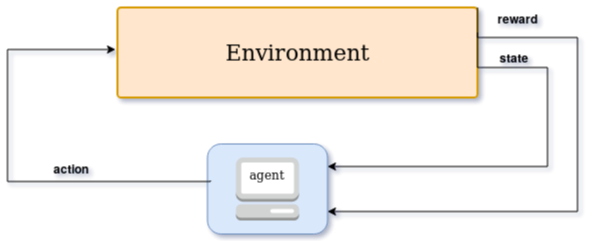
\includegraphics[width=90mm]{bilder/RLFramework.png}
\caption{Agent interacting with the environment}
\end{figure}


\subsection{Elements of Reinforcement Learning}
\citet{Sut98} names 4 other core elements of the reinforcement learning framework.

\textbf{Policy}

The behaviour of the agent at any given time $t$ is determined by the \textit{policy}. A policy $\pi$ can roughly be described as a mapping of states to an action or a distribution over actions. 
We denote the probability of an action $a$ being taken at state $s$ at time $t$ under a policy $\pi$ as $ \pi(a \mid s_t) $ 
Within this work, the policy is always stochastic and the probability distribution over actions is denoted as $\pi (\bullet \mid s)$

\textbf{Reward Signal}

The problem posed by an environment is defined through the reward function. 
The goal of the learning agent is to receive the maximum accumulated future reward at any given time. One of the most important features of reinfocement learning is the fact, that rewards are often very delayed. Connecting the delayed reward with the actions that caused it is a key task of reinforcement learning.
Good examples are games like Pong or Breakout, where the reward is caused by successfully playing a ball, but only received many frames later.

Games like chess pose an even bigger problem, since every move can play an important role in winning the game. Good opening moves can strongly impact if the game is lost or won 100 moves later.
The reward received by an agent at timestep $t$ will be denoted as $r_t$.

\textbf{Value Function}

The value of a state describes how much more reward can be earned from this state onwards. Values represent the sum of the future rewards, and indicate the long term desirability of states.

The value of a state at timestep $t$ under a policy $\pi$ is given through the Expentancy of the \textit{Return} $R_t$ , which is the possible accumulated future reward denoted as $V(s)$ and given by:

\begin{equation}
{
V^\pi (s) = E_\pi \{R_t \mid s_t = s\} = E_\pi \left\{ \sum_{k=0}^\infty \gamma^k r_{t+k+1} \mid s_t = s \right\}
}
\end{equation}

In accordance with this, we define the state-action value $Q(s,a)$, which is simply the expected return, if the action $a$ is taken at state $s$.

\begin{equation}
{
Q^\pi (s,a) = E_\pi \{R_t \mid s_t = s, a_t = a\} = E_\pi \left\{ \sum_{k=0}^\infty \gamma^k r_{t+k+1} \mid s_t = s, a_t = a \right\}
}
\end{equation}

This is a good place to additionally define the advantage $A^\pi(s,a)$ of  $s$ given $a$ is taken.

\begin{equation}
A(s,a) = Q(s,a)-V(s,a)
\label{adv}
\end{equation}

The advantage of an action given a state denotes, how much better this action is, compared to the average action.

\textbf{Environment Model}

In order to solve a problem, a model of the environment can be learned and used for planning. A model can be used to predict future states and rewards before they happen.
Model-based and model-free reinforcement learning methods, which explicitly learn by trial and error both play an important role in reinforcement learning.

Within this thesis we will only look at model-free methods. Rather than learning a model, the agent learns directly through trajectories sampled from the environment.

\pagebreak

\subsection{Markov Decision Process} 

The sequential decision making process of the \textit{agent} can be more formally described as a Markov decision process (MDP).

The sequential decision making process is given by a sequence of states, actions and rewards:

$S_0, A_0, R_0, S_1, A_1, R_1, S_2, A_2, R_2, \dots, S_t,A_t,R_t, S_{t+1}$

Within this thesis a finite environment is assumed. We call a state \textit{Markov} or say it has \textit{Markov property} if it only depends on it's predecessor rather than the whole history.
\begin{equation}
P(s_{t+1} = s', r_{t+1} = r' \mid s_t, a_t, r_t, s_{t-1}, \dots ,r_1,a_0,s_0) = P(s_{t+1} = s', r_{t+1} = r' \mid s_t,a_t)
\end{equation}

A finite discounted Markov decision process $MDP(S,A,P_a,R_a,\gamma)$ contains a finite set of states $S$, 
a finite set of actions $A$,
the transition probablity to end up in state $s'$ if action $a$ is taken in state $s$ : 
\begin{equation}
P^a_{s s'} = Pr(s_{t+1} = s' \mid s_t = s, a_t = a)
\end{equation}

the reward function $R^a_{s s'}$,
and the discount factor $\gamma  \in [0,1)$, used to define the importance of immediate reward in contrast to future reward. 

\subsection{Deep Reinforcement Learning}
In contrast to simply mapping an input to an output value, deep learning algorithms contain so called \textit{hidden layers}.


Usually a transformation or activation function is used on the input. Rectified linear units (ReLU), the tanh or the sigmoid function can be named as popular activaton functions.
After feeding an input into the network and calculation an error value, the weights are adjusted through backpropagation.

Convolutional neural networks (CNN) were inspired by visual neuroscience and are great tools to process image data. CNNs usually contain convolutional layers, pooling layers and fully connected layers.
Other relevant approaches are recurrent neural networks (RNN) or long short term memory networks (LSTM). Both mimic functions of a memory and have started to play bigger roles within the field of deep reinforcement learning recently.

Combining deep learning methods with reinforcement learning methods was a major breakthrough, enabeling reinforcement learning methods to be successfully applied to complex problems like those posed by the Atari 2600 console. \citep{deeprlLi}

Within this thesis, we will only work with CNNs, consisting of convolutional layers, dense layers and ReLU activation functions.

We use convolutional data to extract features from images. By moving a filters over the image, the weight values of the filter are multiplied with the pixel data provided by the part of the image.

The output is a weighted sum of a part of the original image.
The \textit{stride} denotes how much a filter is shifted before being applied to the image again. Usually many filters are used, to receive many different features.

\begin{figure}
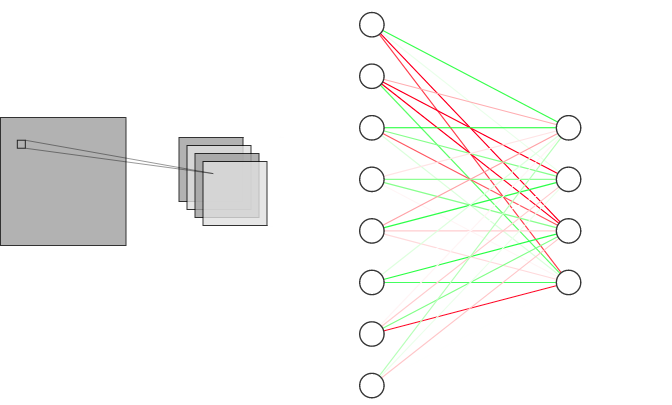
\includegraphics[scale=0.5]{bilder/deeplayers.png}
\caption{A convolutional (left) and fully connected (right) layer.
}
\end{figure}

Fully Connected Layers are used to weight the input data and map it to the output space. Each 'Neuron' or Element in the output layer, hold a weighted sum of every input element.

The ReLU function simply changes all negative values to 0, while positive values remain untouched:

\begin{equation}
ReLU (x) = 
\begin{cases}
x & \text{if x >0} \\
0 & else
\end{cases}
\end{equation}


\pagebreak
\section{Actor-Critic Methods}
\raggedbottom 
Many different approaches to different kind of reinforcement learning problems exist. 
Dynamic programming methods can compute optimal policies, however a perfect model of the environment as MDP is required.
Monte-Carlo methods on the other hand can estimate value functions and discover optimal policies by averaging over sampled trajectories.

\subsection{Monte-Carlo Predictions}

We call a complete run of the environment from start to termination an \textit{episode}.
Monte-Carlo predictions learn from complete episodes. They can be used to estimate the value of a state by calculating the discounted returns for every encountered state and changing the estimated value of the states slightly in the direction of the discounted return.

MC-methods learn relatively fast, however each update requires a full episode.

\subsection{TD-Learning}

\cite{Sut98} describes \textit{temporal difference} (TD) learning as one of the central ideas in reinforcement learning.
TD learning combines dynamic programming and Monte-Carlo ideas to learn eather \textit{state-values: V(s)} or \textit{state-action values: Q(s, a)}
Just like Monte-Carlo methods, TD-learning can learn directly from experience, while being able to learn without the need of finishing an episode through bootstrapping.

We will take a look at the most basic TD method for learning a value function. 
The update step is given as:

\begin{equation}
V(s_t)\gets V(s_t)+ \alpha [r_{t+1} + \gamma V(s_{t+1})-V(s_t)]
\end{equation}

Another popular TD-Method is Q-Learning.
It is used to estimate the state-action value function $Q$, and has a similar update step:

\begin{equation}
Q(s_t,a_t)\gets Q(s_t,a_t)+ \alpha [r_{t+1} + \gamma \max_a Q(s_{t+1},a)-Q(s_t,a_t)]
\end{equation}

After learning a Q-function, the agent has a reliable method to estimate and maximize the return, considering the learned function resembles the \textit{true state-value function} $Q*$ close enough. 
A common approach to achieve this is the use of a $\epsilon$-greedy policy, where a gradually decreasing value ($\epsilon$) is used to decide if a random action or the action assumed to be the best by the learned function is taken. This ensures both sufficient exploration and  exploitation, as it starts with a (mostly) random policy, and ends up with a deterministic policy always choosing the action with the highest estimated return.\citet{Sut98}

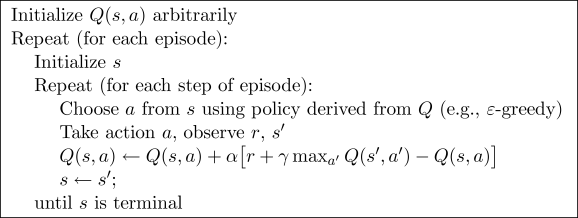
\includegraphics[scale=0.5]{bilder/qlearning2.png}

\caption{Q-learning algorithm taken from \citep{Sut98}}

\subsection{N-Step TD-Learning}

The TD-Learning algorithm shown only learns from a single step. Often episodes and be long, and the final reward (e.g. winning or losing a game) can be very important. 1-step learning can take a very long time to propagate this final reward into earlier states. In general TD-Learning is rather slow, compared to learning from full returns.

We can approach this problem by using n-step TD-learning.
Note that '$\inf$-step' TD update would be the same as a Monte-Carlo updates.

By combining the Monte-Carlo target
\begin{equation}
R_t = r_{t+1}+\gamma r_{t+2}+\gamma^2 r_{t+3}+\gamma^3 r_{t+4}++\gamma^T-t-1 r_{T}
\end{equation}

 ($T$ denotes the final step of the episode) with the TD approach, we can define the n-step TD-learning update:
 
\begin{equation}
V(s_t) = V(s_t) + \alpha(\gamma^nV(s_{t+n}+R_{t:t+n} - V(s_t)
\end{equation} 

where 

\begin{equation}
R_{t:t+n} = r_{t+1}+\gamma r_{t+2}+\gamma^2 r_{t+3}+ \dots +\gamma^{n-1} r_{t+n}
\end{equation}

denotes the discounted return for the next n steps.
\subsection{Critic-Only Methods}

The shown Q-learning algorith or SARSA are popular critic-only methods.

Critic-only methods learn state-action values. They do not contain an explicit function for the policy, but rather derive it from the learned state-action values by acting greedy on the Q-Values.

Critic-olny methods provice a low variance estimate of the expected returns, however the methods suffer from being biased and can be problematic in terms of convergence.

\subsection{Actor-Only Methods}

Onlike critic-only methods, actor only methods do not learn any state or state-action values.
Instead they perform optimization directly on the policy.
Usually a stochastic and parameterized policy $\pi_\theta$ is used.

Policy gradient methods like REINFORCE change the policy in order to maximize the average reward at a given timestep by performing gradient ascent. \citep{Williams1992}
We define an objective function $J(\theta)$ which is a measurement of performance.

The learning agent seeks to maximize $J(\theta)$ through gradient ascent

\begin{equation}
\theta_{t+1} = \theta_t + \alpha \widehat{\nabla J(\theta_t)}
\end{equation}

where $\widehat{\nabla J(\theta_t)}$ denotes an approximated gradient of the performance measure.
Methods of this schema are policy gradient methods \citep{Sut98} 

For the episodic case we define $J(\theta)$ to be the initial value of our policy. We should note that this only works under the assumption, that the environments always provides the same initial state.

\begin{equation}
J(\theta) \doteq v_{\pi_\theta}(s_0)
\end{equation}

We can approximate the gradient of $J(\theta)$ , $ \nabla v_{\pi_\theta}(s_0)$ through

\begin{equation}
\nabla J(\theta) \propto \sum_s \mu (s) \sum_a q_\pi (s,a) \nabla_\theta \pi(a \mid s, \theta)
\end{equation}

thanks to the policy gradient theorem. The proof for this theorem can be found in the reinforcement learning book by \citet{Sut98}.

$\mu$ denotes the on-policy distribution under $\pi$.

However if trajectories are sampled on-policy, we can simply rewrite this as the expectation under policy $\pi$:

\begin{equation}
\nabla J(\theta) \propto E_\pi \left[ \sum_a q_\pi (s_t,a) \nabla_\theta \pi (a \mid s_t, \theta) \right]
\end{equation}




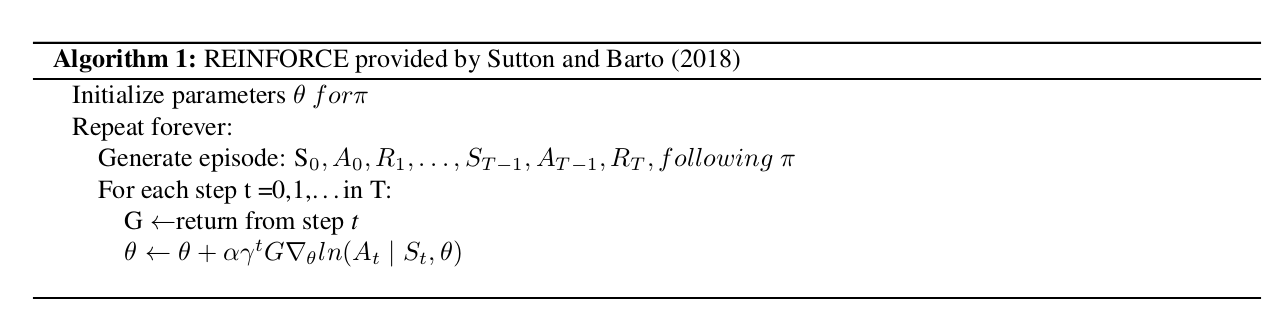
\includegraphics[scale=0.4]{bilder/REINFORCE.png}


In contrast to value based approaches, policy gradient methods provide strong convergence to at least a local maximum.
On top of that, actor methods are applicable on continuus action spaces.
 \citep{Sutton00policygradient}
 
Actor-only methods however suffer from a large variance of the gradient. Compared to critic-only methods their learning process is significantly slowed down. \citep{Grondman12}
 

\subsection{Actor-Critic Methods}

Actor-critic methods tackle the problem of high variance in policy gradient methods with the use of a critic.

They combine the strenght of both approaches to achieve a learning agent, which has strong convergence, yet low variance.

Since actor-critic methods are still policy gradient methods at their core, they provide the possibility to work on continuous actions spaces just like the actor-only approach.

The main reason for the variance in the gradient is the high variance of the return. By introducing a baseline $ b(s)$, to the objective function, we can achieve a lower variance, without creating bias.
The idea behind this is to increase the probability of an action in relation to how much better it is compared to other actions at this state, rather than the full return.

\begin{equation}
\nabla J(\theta) \propto \sum_s \mu(s) \left[ \left( \sum_a q_\pi (s,a) -b(s)\right) \nabla_\theta \pi (a \mid s, \theta) \right]
\end{equation}

The term $q_\pi(s_t,a) -b(s)$ can be replaced by different terms \citep{Schulman15}.
Popular choices for actor-critic learning are the advantage function $A_\pi$ (\ref{adv}) or the TD residual 

\begin{equation}
r_t + V_\pi(s_{t+1}) - V_\pi(s_t)
\end{equation} 



\begin{figure}
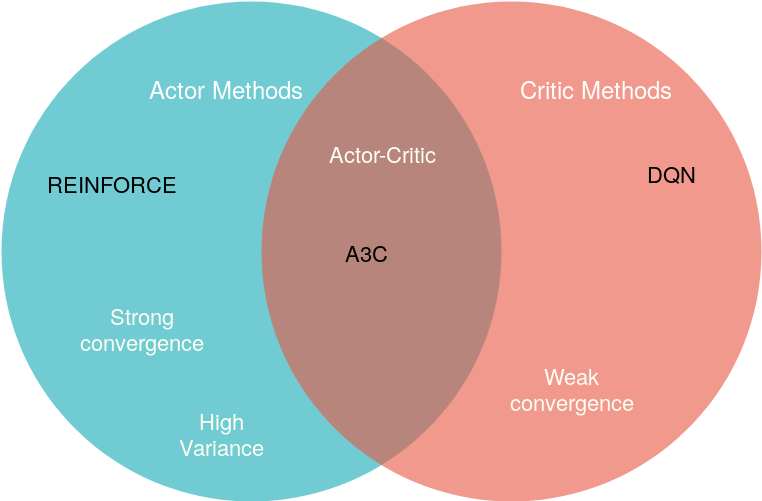
\includegraphics[scale=0.5]{bilder/actorcritic1.png}
\caption{Actor, Critic, and Actor-Critic approach}
\end{figure}

\pagebreak



\subsection{Asynchronous Advantage Actor Critic (A3C)}

In general we call an algorithm on policy, if the data used in the policy update was sampled under the same policy. The sequence of observed data encountered by an RL agent is strongly correlated and non-stationary \citep{A3C}. This can have a negative influence on the learning process.

Previous methods usually approached this problem by using randomly selected samples from a replay memory. \citep{mnih2015atari}

Training an agent comes with a high demand for computational power. To achieve feasible training times, former algorithms heavily relied on a strong GPU.

The asynchronous advantage actor critic(A3C) algorithm solves both problems, by training simultaneously on multiple environment.
Each learner samples trajectories and computes gradients. Those gradients are then applied to the shared parameters. 
After each global update step, the local parameters are synchronized.
This method not only enables efficient CPU computation with multiple threads, rather than requiring a strong GPU, but solves the problem of correlation since every environment can be assumed to be in different states.
Usually 16 or 32 environments are used, to ensure the decorrelation of the samples.

A3C samples trajectories of length $n$ and uses the longest possible k-return for the update step, meaning the last state uses a one-step update, the second to last a two-step update and so on, with the first state using an n-step update.
The gradients are accumulated over all state withing the trajectory and applied in a single gradient step. 

\begin{figure} 
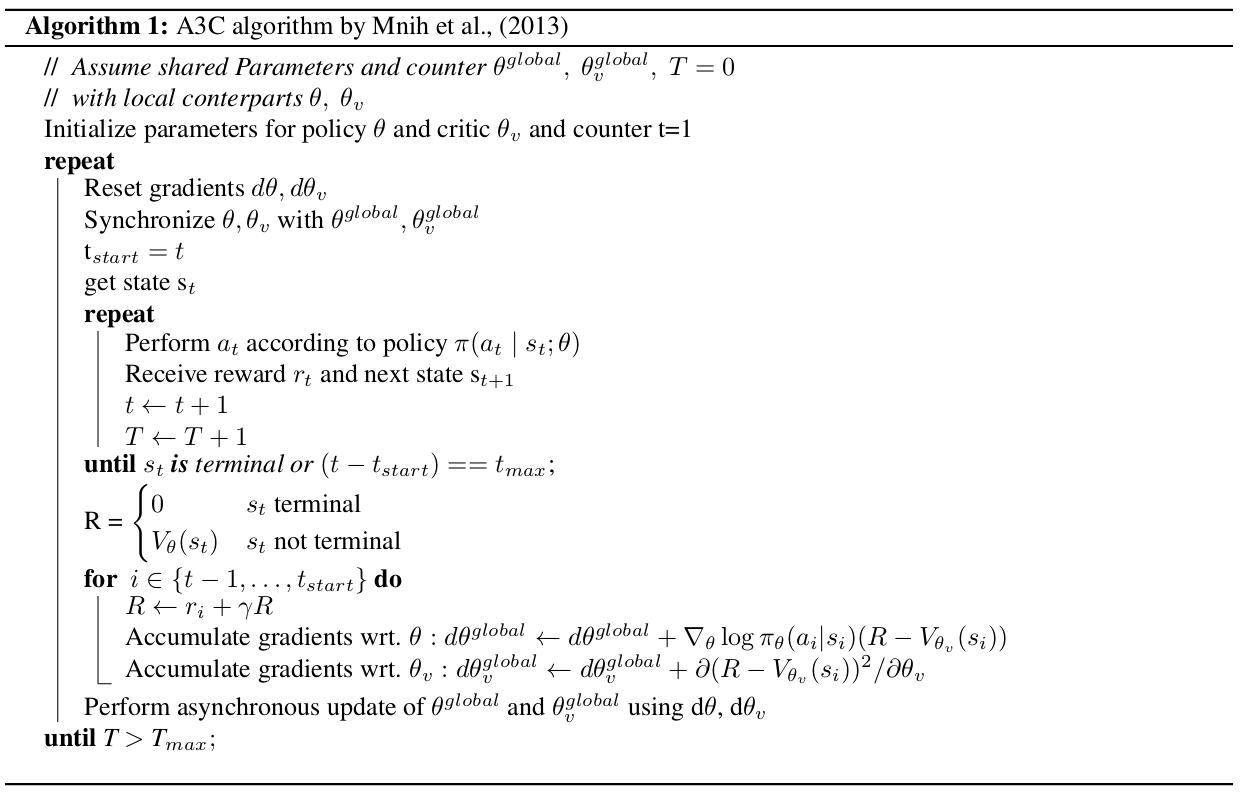
\includegraphics[scale=0.3]{bilder/aaac.png}
\caption{A3C by \citet{A3C}}
\end{figure}
\pagebreak
\section{Off-Policy Learning}
\raggedbottom 

Off-policy methods use data previously sampled under a so-called \textit{behavior policy} denoted as $\mu(a \mid s)$  which is different to the \textit{current/target policy}  $\pi$ that is optimized.

One benefit of off-policy learning is the possibility to chose a more exploratory behaviour policy. 
Another benefit is the possibility to increase sample efficiency by reusing old data.
\citep{Degris12}

Off-policy methods can have the drawback of being divergent.
The class of asynchronous methods A3C belongs to is always slightly off-policy, but since the behaviour policy is close enough to the target policy, the influence is neglectable

Whenever the behaviour policy differs too much from the target policy, the algorithm can no longer be viewed as \textit{safe} without correcting for the 'off-policyness'. \citep{Munos16}

Ensuring convergence even for an arbitrary level of 'off-policyness' is a problem addressed by a multitude of methods.
We will look at the most important ones, leading up to the retrace-algorithm used for our experiments.

\subsection{Importance Sampling (IS)}

One of the most basic ideas is to correct for the "off-policyness" by using importance sampling (IS).
It is a classic and well-known technique for estimating the value of a random variable $x$ with distribution $d$  if the samples were drawn from another distribution $d'$
by using the product of the likelihood ratios.

In regards to $\pi$ and $\mu$, the importance weight is denoted as

\begin{align}
{
p_t = \frac{\pi (a_t \mid s_t)}{\mu (a_t \mid s_t)}.
}
\label{IW}
\end{align}
Even though this method can guarantee convergence \citep{Munos16} for arbitrary $\pi$ and $\mu$, it comes with the risk of high, possible infinite  variance, due to the variance of the product of importance weights.

\subsection{Tree-backup, TB(\lambda)}

The tree-backup method allows off-policy corrections, without the use of importance sampling by using estimated values of untaken actions as an offset to the rewards from the off-policy sample. \citet{Precup00}

The algorithm provides low variance off-policy learning with strong convergence.
However if a sample is drawn from a policy which is close to the target policy, the algorithm unnecessarily cuts the traces. Without using the full returns, the learning process is slowed down.
\pagebreak
\subsection{Retrace($\lambda$)}

\citet{Munos16} introduced the retrace($\lambda$) algorithm. By combining ideas of importance sampling and tree-backup, a method with strong convergence, yet low variance was achieved that is still able to use the benefits of full returns.

Similar to how it is done in TB($\lambda$), the traces are safely cut in case of strong "off-policyness", but without impacting the update too much, if the data was sampled under a behaviour policy $\mu$ close to the target policy $\pi$.

Retrace values for a q funcion are obtained recursively by

\begin{align}
{
Q^{ret}(x_t,a_t)=r_t+\gamma \tilde{p}_{t+1} [Q^{ret}(x_{t+1},a_{t+1} ) -  Q(x_{t+1},a_{t+1})] + \gamma V(x_{t+1})
}
\label{qretrace}
\end{align}

with $\tilde{p} = min\{c,p_t\}$ being the truncated importance weight $p_t$ (\ref{IW}).

In case of a terminal state, the retrace value is equal to the final reward.
Note that the formula is given considering $\lambda = 1$

As $\lambda = 1$ performs the best for the Atari console games \citep{Munos16}, other values were not considered within this Thesis.

\pagebreak

\section{Actor-Critic with Experience Replay (ACER)}
\raggedbottom 

"Actor critic with experience replay" (ACER) introduced by \citet{ACER} was one of the first approaches to create a sample efficient, yet stable actor critic method, that applies to both contiuous and discrete action spaces.

ACER combines recent breakthroughs in the field of RL, by utilizing both the ressource efficient parallel training of RL agents proposed by \citet{A3C} and the Retrace algorithm \citep{Munos16}.

These approaches were combined with truncated importance sampling with bias correction and an efficient trust region policy optimization.
For continuous action spaces, stochastic dueling network architectures were used.

Acer can be viewed as an off-policy extension of A3C \citep{A3C}.

The importance weighted policy gradient is given by:
\begin{align}
\hat{g}^{imp} = \left(\prod^k_{t=0}p_t\right) \sum^k_{t=0}\left(\sum^k_{i=0}\gamma^ir_{t+i}\right) \nabla_\theta \ log \ \pi (a_t \mid s_t)
\end{align}

The unbounded importance weights can cause massive variance. \citet{Degris12} approached this problem by approximating the policy gradient as

\begin{align}
g^{marg} = E_{s_{t \textasciitilde{}} \beta, a_{t \textasciitilde{}} \mu} \left[p_t \nabla_\theta log \pi_\theta(a_t \mid s_t) Q^\pi (s_t,a_t) \left]
\end{align}

where $\beta$ denotes the limiting distribution and behaviour policy $\mu$

To compute this gradient, knowledge about $Q^\pi$ is nessecary. The retrace values (\ref{qretrace}) present a good estimation for $Q^\pi$.

To further reduce the variance, the importance weights are truncated.
A core problem of actor-critic methods is the tradeoff between bias and variance. By truncating the importance weights, bias is introduced.
To counter this, ACER uses a bias correction term.

The final ACER policy gradient is given as:

\begin{equation}
\begin{split}
g^{ACER}_t = \tilde{p}_t \nabla_\theta log \pi_\theta(a_t \mid s_t) \left[Q^{ret}(s_t,a_t) - V_\theta_v(s_t)\right] \\
+ E_{a_{\textasciitilde{}\pi}} \left(\left[\frac{p_t(a) -c}{p_t(a)\right]}_+ \nabla_\theta log \pi_\theta(a \mid s_t) \left[Q_\theta_v(s_t,a) - V_\theta_v(s_t)\right]\right)
\end{split}
\end{equation}

The critic $Q_\theta_v$ is trained by minimizing the mean squared error with the retrace values as the target.

\citet{ACER} proposed an efficient trust region policy optimization (TRPO), which limits the update step in a way, that the new policy doesnt deviate too much from an average policy. 
\pagebreak

Even though the improvement through the TRPO method on the continuous action space environments was significant, the results presented in the paper only showed a marginal improvement for discrete action space environments.
Because all experiments in this thesis are on discrete action space in order to run more experiments the TRPO was not used.

\subsection{Experimental Setup}

\subsubsection{Environment}
All experiments were made using multiple selected games from the Atari 2600 console game environments providede by \citet{openaigym}.

In our experiments the following OpenAI-Gym environments were used:

\textbf{Breakout} is a game that rapidly speeds up, making it easy for machines to show "superhuman" performance.

\textbf{Seaquest} poses a serious problem for learning agent, as they tend to get stuck on local maxima. It is especially interesting, as it provides multiple possibilities to achieve rewards, and the loss of the game if the player runs out of oxygen is a game mechanic a human can grasp in seconds, while it is notoriously hard for reinforcement learning agents to 'understand'.

Scoring well on this environment can be considered a great achievement.

\textbf{Space Invaders} is a fast paced game. Human and reinforcement learning approaches usually have similar scores. \citep{mnih2015atari}

The hyperparameters were adjusted to ensure a good performance for the Breakout environment. Test on other environments were all performed with the same set of hyperparameters.


OpenAI gym environments provide the agent with a 210x160 pixel colored image. An \textit{environment step} consist of frame skipping, which means, that the action fed into the environment is repeated for k frames. Where k denotes a random number within $\{2,3,4\}$.
\subsubsection{Preprocessing}
Using full scale colored images would come with huge computational cost. To be able to work with the data, each frame is preprocessed.
After grayscaling and transforming the frame, the scoreboard area is chopped off. With this method a 84x84 grayscaled pixel image is obtained. 

\citet{nature} proposed to stack multiple frames. More specifically the state contains the last 4 frames received and therefore has a shape of 84x84x4.

To receive the initial state, we simply stack the first frame 4 times.

\begin{figure}
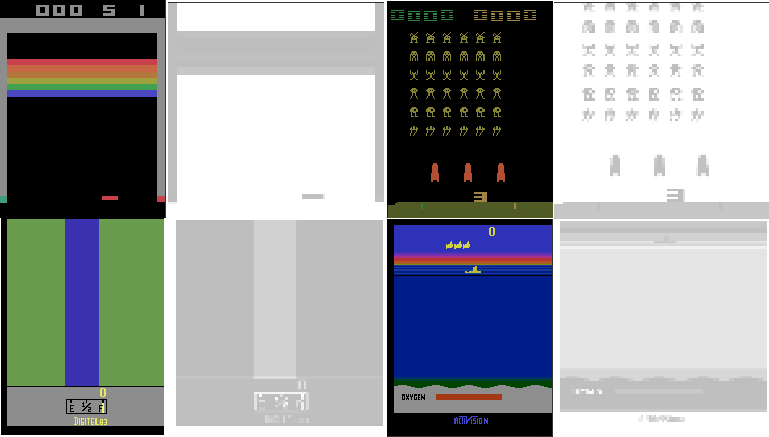
\includegraphics[scale=0.5]{bilder/atarienv.png}
\caption{The Atari 2600 console games Breakout, SpaceInvaders, Riverraid and Seaquest before and after being processed.}
\end{figure}

\subsubsection{network architecture}

Two architectures were tested. \citep{mnih2015atari} \citep{nature}.

Both provided good results. Since the paper uses the architecture proposed in the nature paper \citep{nature}, all further experiments were done using this architecture.

Similar to the \citep{A3C} network, most of the parameters are shared and used for both estimating $Q^\pi$ and to output a policy.

The shared net consists of 3 convolutional layers.
First 32 8x8 filters are applied with a stride of 4.
The 2nd layer consists of 64 4x4 filters using a stride of 2.
The last convolutional layer uses 64 3x3 filters with stride 1.
Finally a fully connected layer of size 512 is applied.

Each of the mentioned layers is followed by a rectifier nonlinearity (ReLU) function, ReLU is used to set all negative outputs to 0, ensuring only positive values are passed to the next layer.
Even though other activation/transformation functions exist, the ReLU has empirically done really well. 

A test run using tanh instead of ReLU caused a strong loss of performance.

The final shared layers is then mapped to the action space twice to obtain the action scores, and the Q-values. We use a softmax policy to receive the distribution over actions.
The action is randomly sampled from the softmax probabilities.

\begin{equation}
P(A = a' | s ) = \frac{e^{z_{a'}}}{\sum^N_{i=0}e^{z_{a_i}}} 
\end{equation}

where $z_{a}$ denotes the score assigned to the action through the last network layer.


\begin{figure}
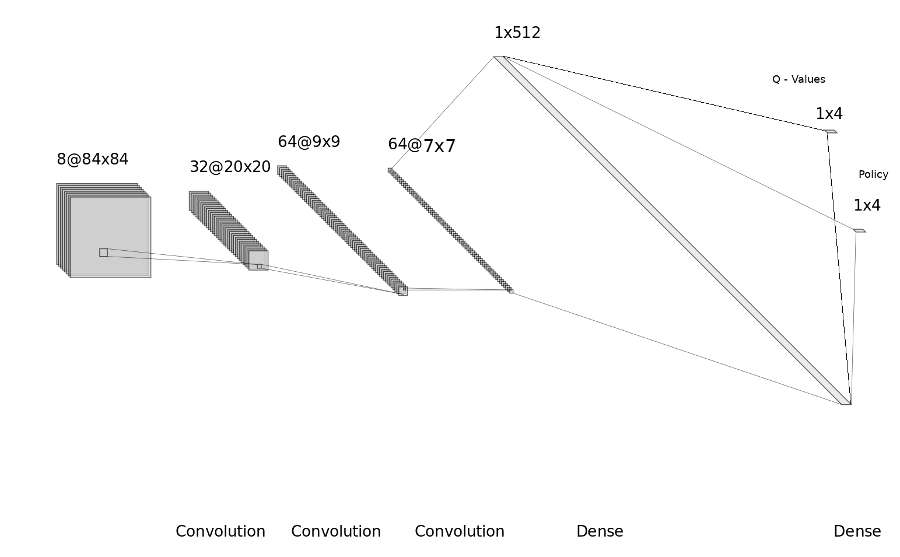
\includegraphics[scale=0.5]{bilder/nn2.png}
\caption{Shared network for policy and Q-Value approximization for an environment with 4 possible actions}
\end{figure}

The agent is trained by using 16 learner threads running on the CPU. Each Thread has it's own replay buffer, which ensures a more balanced replay and reduces the risk of a single trajectory being used unreasonably often compared to a single shared replay buffer.

Updates to the network were performed every 20 steps or if the environment reached a terminal state. 

Replay buffers were designed to hold up to 2500 trajectories, therefore ~50.000 frames were saved for each thread and $_\tilde{}$ 800.000 frames were stored in total, which is the same size used by DQN \citep{nature}}

If no replay is used, ACER essentially becomes a version of A3C which uses retrace and Q-values, rather than learning the value function. \citep{A3C}

For the offline setting, replay ratios of 1,2 and 4 were considered, where a ratio of 4 would mean, that the net is trained on trajectories sampled from the replay buffer 4 times for every online update.




%%%%%%%%%%%%%%%%%%%%%%%%%%%%%%%%%%%%%%%%%%%%%%%%%%%%%%%%%%%%%%%%%%%%%%%%
%%%% ENDE TEXTTEIL %%%%%%%%%%%%%%%%%%%%%%%%%%%%%%%%%%%%%%%%%%%%%%%%%%%%%
%%%%%%%%%%%%%%%%%%%%%%%%%%%%%%%%%%%%%%%%%%%%%%%%%%%%%%%%%%%%%%%%%%%%%%%%

\clearpage

% Entfernen Sie das Kommentar aus der nachfolgenden Zeile, falls Sie einen Anhang in der Arbeit verwenden wollen. Beachten Sie, dass Sie sich im Verlauf der Arbeit mit \ref{...} (z.B. \ref{anhang:zusatz1}) auf den Anhang beziehen.
%\newpage
\appendix
\section{Anhang}

\subsection*{Zusatzteil 1} \label{anhang:zusatz1}

Dies ist ein Anhang.

\clearpage

%\bibliography{references}
%\bibliographystyle{alphadin}
\DeclareNameAlias{sortname}{first-last}
\printbibliography[heading=bibintoc, title=References]
%\vspace*{\fill}

\clearpage

\listoffigures

\listoftables

%\pagebreak

%\printindex
\end{document}
